\documentclass[letterpaper, 10 pt, journal, twoside]{IEEEtran}
\IEEEoverridecommandlockouts

% Quarto basics minus two problematic packages
\RequirePackage{scrlfile}
\PreventPackageFromLoading{sidenotes}
\PreventPackageFromLoading{marginnotes}


\providecommand{\tightlist}{%
  \setlength{\itemsep}{0pt}\setlength{\parskip}{0pt}}\usepackage{longtable,booktabs,array}
\usepackage{calc} % for calculating minipage widths
% Correct order of tables after \paragraph or \subparagraph
\usepackage{etoolbox}
\makeatletter
\patchcmd\longtable{\par}{\if@noskipsec\mbox{}\fi\par}{}{}
\makeatother
% Allow footnotes in longtable head/foot
\IfFileExists{footnotehyper.sty}{\usepackage{footnotehyper}}{\usepackage{footnote}}
\makesavenoteenv{longtable}
\usepackage{graphicx}
\makeatletter
\def\maxwidth{\ifdim\Gin@nat@width>\linewidth\linewidth\else\Gin@nat@width\fi}
\def\maxheight{\ifdim\Gin@nat@height>\textheight\textheight\else\Gin@nat@height\fi}
\makeatother
% Scale images if necessary, so that they will not overflow the page
% margins by default, and it is still possible to overwrite the defaults
% using explicit options in \includegraphics[width, height, ...]{}
\setkeys{Gin}{width=\maxwidth,height=\maxheight,keepaspectratio}
% Set default figure placement to htbp
\makeatletter
\def\fps@figure{htbp}
\makeatother
\newlength{\cslhangindent}
\setlength{\cslhangindent}{1.5em}
\newlength{\csllabelwidth}
\setlength{\csllabelwidth}{3em}
\newlength{\cslentryspacingunit} % times entry-spacing
\setlength{\cslentryspacingunit}{\parskip}
\newenvironment{CSLReferences}[2] % #1 hanging-ident, #2 entry spacing
 {% don't indent paragraphs
  \setlength{\parindent}{0pt}
  % turn on hanging indent if param 1 is 1
  \ifodd #1
  \let\oldpar\par
  \def\par{\hangindent=\cslhangindent\oldpar}
  \fi
  % set entry spacing
  \setlength{\parskip}{#2\cslentryspacingunit}
 }%
 {}
\usepackage{calc}
\newcommand{\CSLBlock}[1]{#1\hfill\break}
\newcommand{\CSLLeftMargin}[1]{\parbox[t]{\csllabelwidth}{#1}}
\newcommand{\CSLRightInline}[1]{\parbox[t]{\linewidth - \csllabelwidth}{#1}\break}
\newcommand{\CSLIndent}[1]{\hspace{\cslhangindent}#1}

\makeatletter
\makeatother
\makeatletter
\makeatother
\makeatletter
\@ifpackageloaded{caption}{}{\usepackage{caption}}
\AtBeginDocument{%
\ifdefined\contentsname
  \renewcommand*\contentsname{Table of contents}
\else
  \newcommand\contentsname{Table of contents}
\fi
\ifdefined\listfigurename
  \renewcommand*\listfigurename{List of Figures}
\else
  \newcommand\listfigurename{List of Figures}
\fi
\ifdefined\listtablename
  \renewcommand*\listtablename{List of Tables}
\else
  \newcommand\listtablename{List of Tables}
\fi
\ifdefined\figurename
  \renewcommand*\figurename{Figure}
\else
  \newcommand\figurename{Figure}
\fi
\ifdefined\tablename
  \renewcommand*\tablename{Table}
\else
  \newcommand\tablename{Table}
\fi
}
\@ifpackageloaded{float}{}{\usepackage{float}}
\floatstyle{ruled}
\@ifundefined{c@chapter}{\newfloat{codelisting}{h}{lop}}{\newfloat{codelisting}{h}{lop}[chapter]}
\floatname{codelisting}{Listing}
\newcommand*\listoflistings{\listof{codelisting}{List of Listings}}
\makeatother
\makeatletter
\@ifpackageloaded{caption}{}{\usepackage{caption}}
\@ifpackageloaded{subcaption}{}{\usepackage{subcaption}}
\makeatother
\makeatletter
\@ifpackageloaded{tcolorbox}{}{\usepackage[many]{tcolorbox}}
\makeatother
\makeatletter
\@ifundefined{shadecolor}{\definecolor{shadecolor}{rgb}{.97, .97, .97}}
\makeatother
\makeatletter
\makeatother

% Common packages
\usepackage[T1]{fontenc}
\usepackage{lipsum}
\usepackage{amsmath}
\usepackage{amssymb}
\usepackage{physics}
\usepackage{siunitx}
\usepackage{graphicx}
\usepackage[hyphens]{url}
\usepackage{threeparttable}
\usepackage{xcolor}
\usepackage{float}
\usepackage{xcolor}
\usepackage{booktabs}
\usepackage{makecell}
\usepackage{orcidlink}
% monofont
\usepackage[scaled=0.8]{inconsolata}

%styled tabled generated from pandas
\usepackage{colortbl}
\usepackage{multirow}
\usepackage{stfloats} % https://tex.stackexchange.com/a/324358

% Fix table in 2-column format and enable wide table
% https://tex.stackexchange.com/a/224096
\makeatletter
% My tables
\newenvironment{mytable}[1][htbp]{
    \begin{figure}[#1]
    \footnotesize
    \onecolumn
    \begin{minipage}{0.5\textwidth}}
{
    \end{minipage}
    \twocolumn
    \end{figure}}

\newenvironment{mywidetable}[1][tbp]{
    \begin{figure*}[#1]
    \footnotesize
    \onecolumn
    \begin{minipage}{1.0\textwidth}}
{
    \end{minipage}
    \twocolumn
    \end{figure*}}

\renewenvironment{table*}{\begin{mywidetable}}{\end{mywidetable}\ignorespacesafterend}
\renewenvironment{table}{\begin{mytable}}{\end{mytable}\ignorespacesafterend}    
\makeatother



% Muted text (for filler text)
\newcommand\muted[1]{%
\bgroup
\hskip0pt\color{black!40!}%
#1%
\egroup
}

% color links
\usepackage{hyperref}
\hypersetup{ colorlinks, citecolor=teal, linkcolor=teal, urlcolor=teal}


\begin{document}

% author blocks
\author{
        Rainer Koelle\(^1\)\orcidlink{0000-0000-0000-0000},     Second
Author\(^1\)\orcidlink{0000-0000-0000-0000},     Third Author\(^2\)
    \thanks{\(^1\)Performance Review Unit, EUROCONTROL. \(^2\)Some
corporation.}
    \thanks{Released on: }
    \thanks{Extra footnote..}
}


% title
\title{Arrival Management with Open Data}
\maketitle

% abstract
\begin{abstract}
    In light of the on-going discussion on climate change, operational
    efficiency of air navigation has gained a higher visibility.
    Efficient operations will positively influence the fuel burn by
    airspace users. While the development and introduction of novel
    aircraft airframe and propulsion technologies, the global pickup
    rate of sustainable aviation fuel, and benefits mechanism of
    market-based measures promise a positive effect over time,
    \textgreater\textgreater{} reducing unnecessary contraints on
    airspace users can be immediately deployed. There is still a
    considerable benefit pool for arrival operations. This
    proof-of-concept paper explores the use of open data for the
    analysis of operational efficiency within the extended terminal
    airspace. To characterise the potentail benefit pool, a method to
    quantify the spacing deviation between successive flights is
    developed. This paper summarises the conceptual approach and reports
    on the first findings of an use-case analysis for a subset of
    European airports. The results show the general feasibility of the
    approach and help to identify requirements for the further
    development of operational performance measures.
\end{abstract}

% body
\hypertarget{introduction}{%
\section{Introduction}\label{introduction}}

Operational efficiency is a key element of addressing aviation's
contribution to climate change. Emissions may increase due to the
expected growth in international air traffic until lower emitting
technologies and fuels and other mitigating measures are developed and
deployed .. ICAO adopted at its 41st Assembly a long-term aspirational
goal for international aviation
\protect\hyperlink{ref-icao2022}{\textbf{icao2022?}}. In support to the
Paris Agreement, the goal is to achieve net-zero carbon emissions by
2050.

Levers for fuel reduction:

* operational efficiency

* market-based measures

* sustainable aviation fuel

* new aircraft propulsion and airframes

A wider use and pick-up of sustainable aviation fuel, and new aircraft
propulsion technologies or aircraft design requires further research.

Despite the introduction of an initial market-based mechanism, immediate
action to curb fuel burn and CO2 emissions rests with improvements of
operational efficiency. ICAO has introduced the trajectory-based
operations concept, which promises operational and environmental
benefits to aviation. where the flight trajectory of an aircraft is
flown as close as possible to the userpreferred route, with as little
disruptions as possible through collaborative decision-making mechanism.
This includes reducing potential conflicts and resolving demand/capacity
imbalances earlier and more efficiently. TBO can therefore bring
significant operational and environmental benefits to aviation.\\

The contribution of this paper comprise:

\begin{itemize}
\item
  conceptualisation of sequencing separation for arrival management and
  development of an open data and open software based implementation of
  the approach; and
\item
  use-case application of the developed approach on a subset of airports
  within the European
\end{itemize}

\hypertarget{trajectory-based-operations---arrival-management}{%
\section{Trajectory-Based Operations - Arrival
Management}\label{trajectory-based-operations---arrival-management}}

Trajectory-based operations (TBO) are a core element of the ongoing
transformation programs for air navigation services (e.g.~Europe/SESAR,
US/Next Gen, Japan/CARATS). On the conceptual level TBO describe a move
from clearance-based operations to a highly predictable and negotiated
trajectory execution between airspace users and air traffic control. The
TBO concept entails the successive refinement (i.e.~negotiation) between
the parties starting from an inital planned trajectory through
operations and the actual execution of flight. TBO builds on higher
levels of information exchange between planning and flow management
systems and the airborne and ground systems during flight operations.
Figure~\ref{fig-TBO-concept} shows the overall timeline and evolution of
a trajectory.

\begin{figure}

{\centering 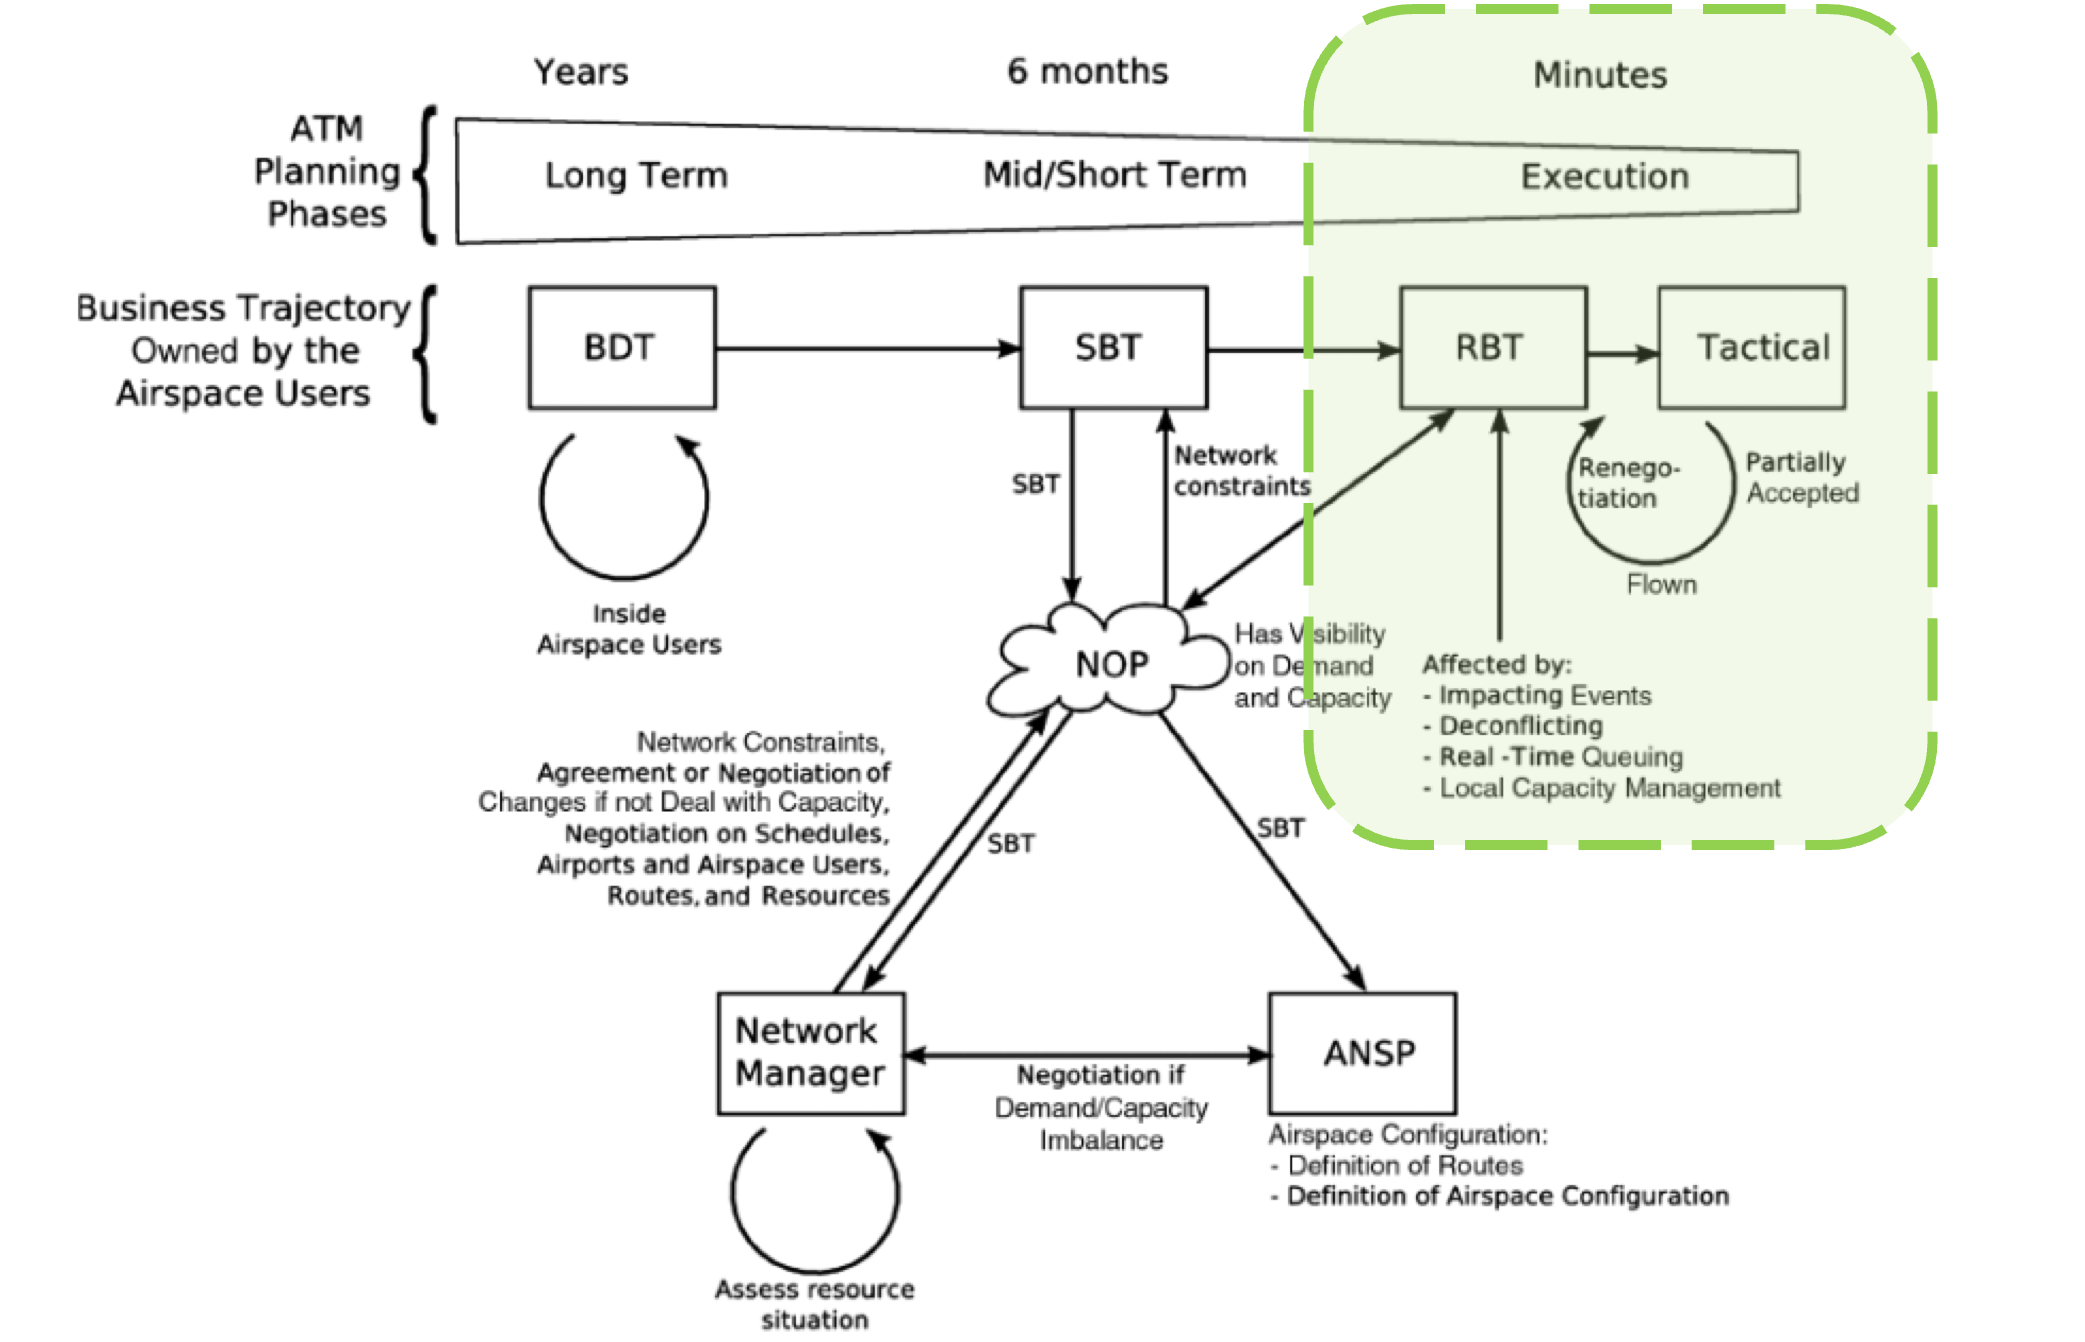
\includegraphics[width=0.45\textwidth,height=\textheight]{./figures/TBO-concept.png}

}

\caption{\label{fig-TBO-concept}Trajectory-based operations - conceptual
perspective}

\end{figure}

For this study we postulate the following goal of trajectory based
arrival management: ``\ldots{} to reduce inefficiencies in the
(extended) arrival phase by establishing an arrival sequence to require
less costly sequencing close to the airport absorbing time/distance in
more fuel efficient altitudes.''

Conceptual approach := technology agnostic CONOPS may entail
technological enablers and/or advanced procedures Performance objectives
observed on concept functional level

\hypertarget{conceptual-approach-and-data}{%
\section{Conceptual Approach and
Data}\label{conceptual-approach-and-data}}

\hypertarget{research-approach}{%
\subsection{Research Approach}\label{research-approach}}

This paper follows an exploratory research process (c.f.
Figure~\ref{fig-research-approach}). We frame the work as a operational
performance analytical problem.

\begin{figure}

{\centering 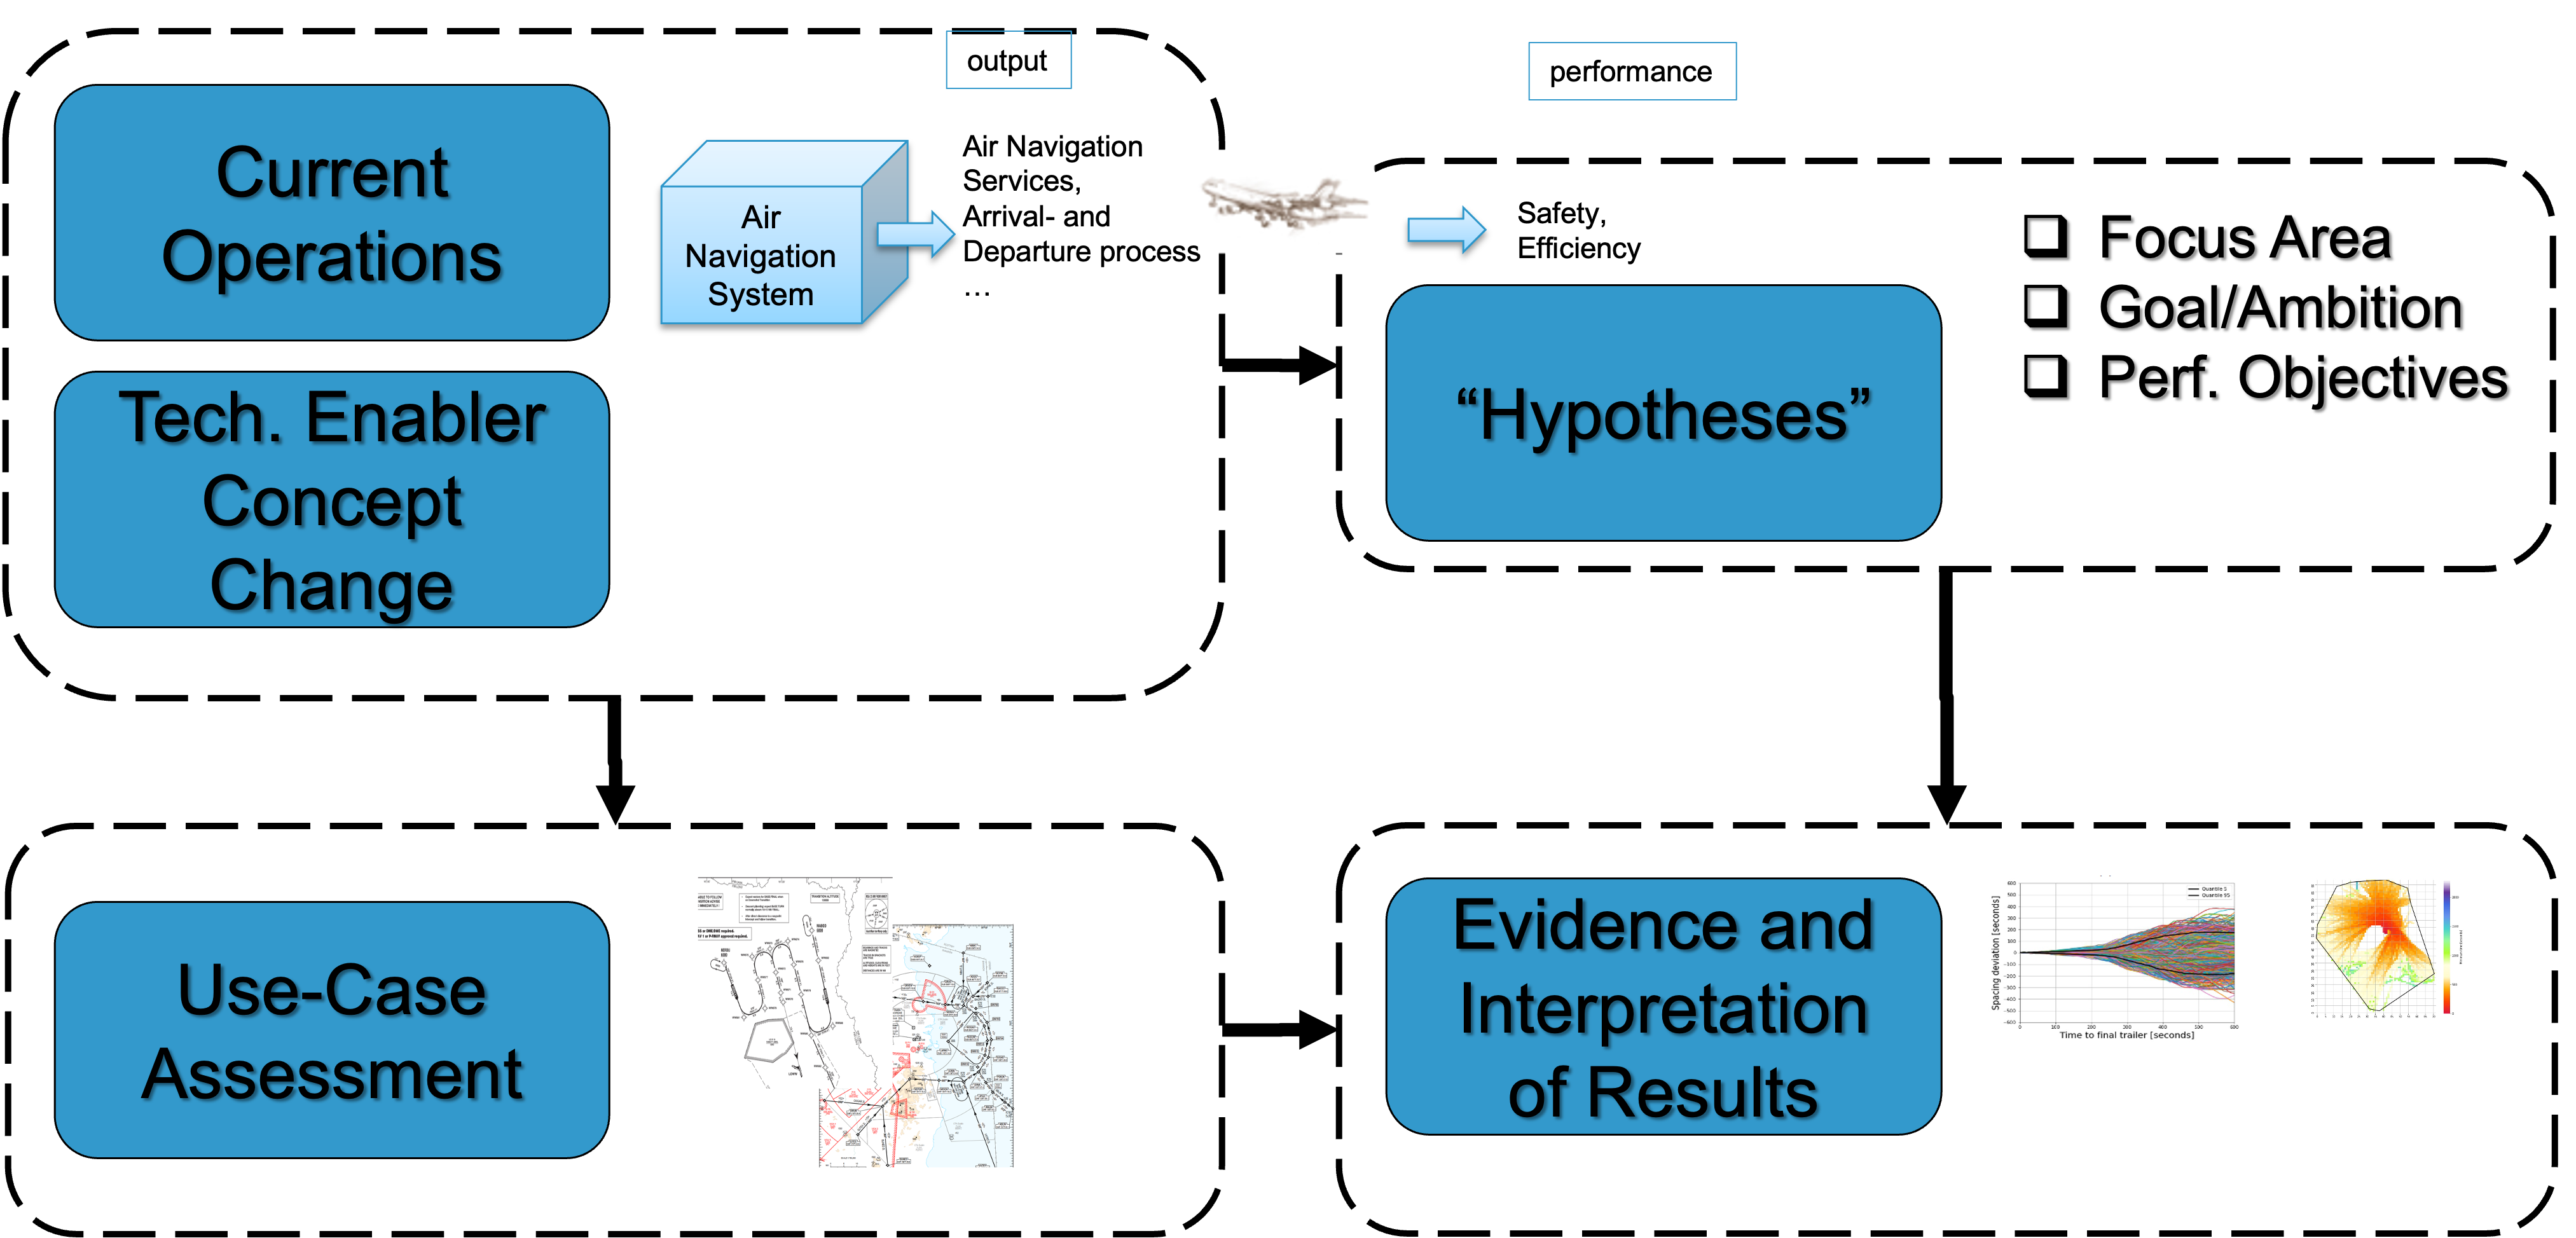
\includegraphics[width=0.45\textwidth,height=\textheight]{./figures/exploratory-research-concept.png}

}

\caption{\label{fig-research-approach}Exploratory research approach}

\end{figure}

\hypertarget{approach}{%
\subsection{Approach}\label{approach}}

data preparation

\begin{itemize}
\tightlist
\item
  trajectory data - Opensky Network, weekly downloads
\item
  airport information - Openstreet Map
\end{itemize}

data downloaded \& script development, data cleaning

\hypertarget{trajectory-flight-phase-segmentation-milestone}{%
\subsubsection{Trajectory Flight Phase Segmentation \&
Milestone}\label{trajectory-flight-phase-segmentation-milestone}}

Different approaches exists to detect and describe aircraft flight
phases, e.g.~recent machine learning algorithm
\protect\hyperlink{ref-sun2017flightphase}{{[}1{]}}. This paper
implements a heuristic approach with a focus on the detection of arrival
traffic at the study airports. Figure Figure~\ref{fig-EGLL-arrivals}
shows the detected arrival flights for a single day.

\begin{figure}

{\centering 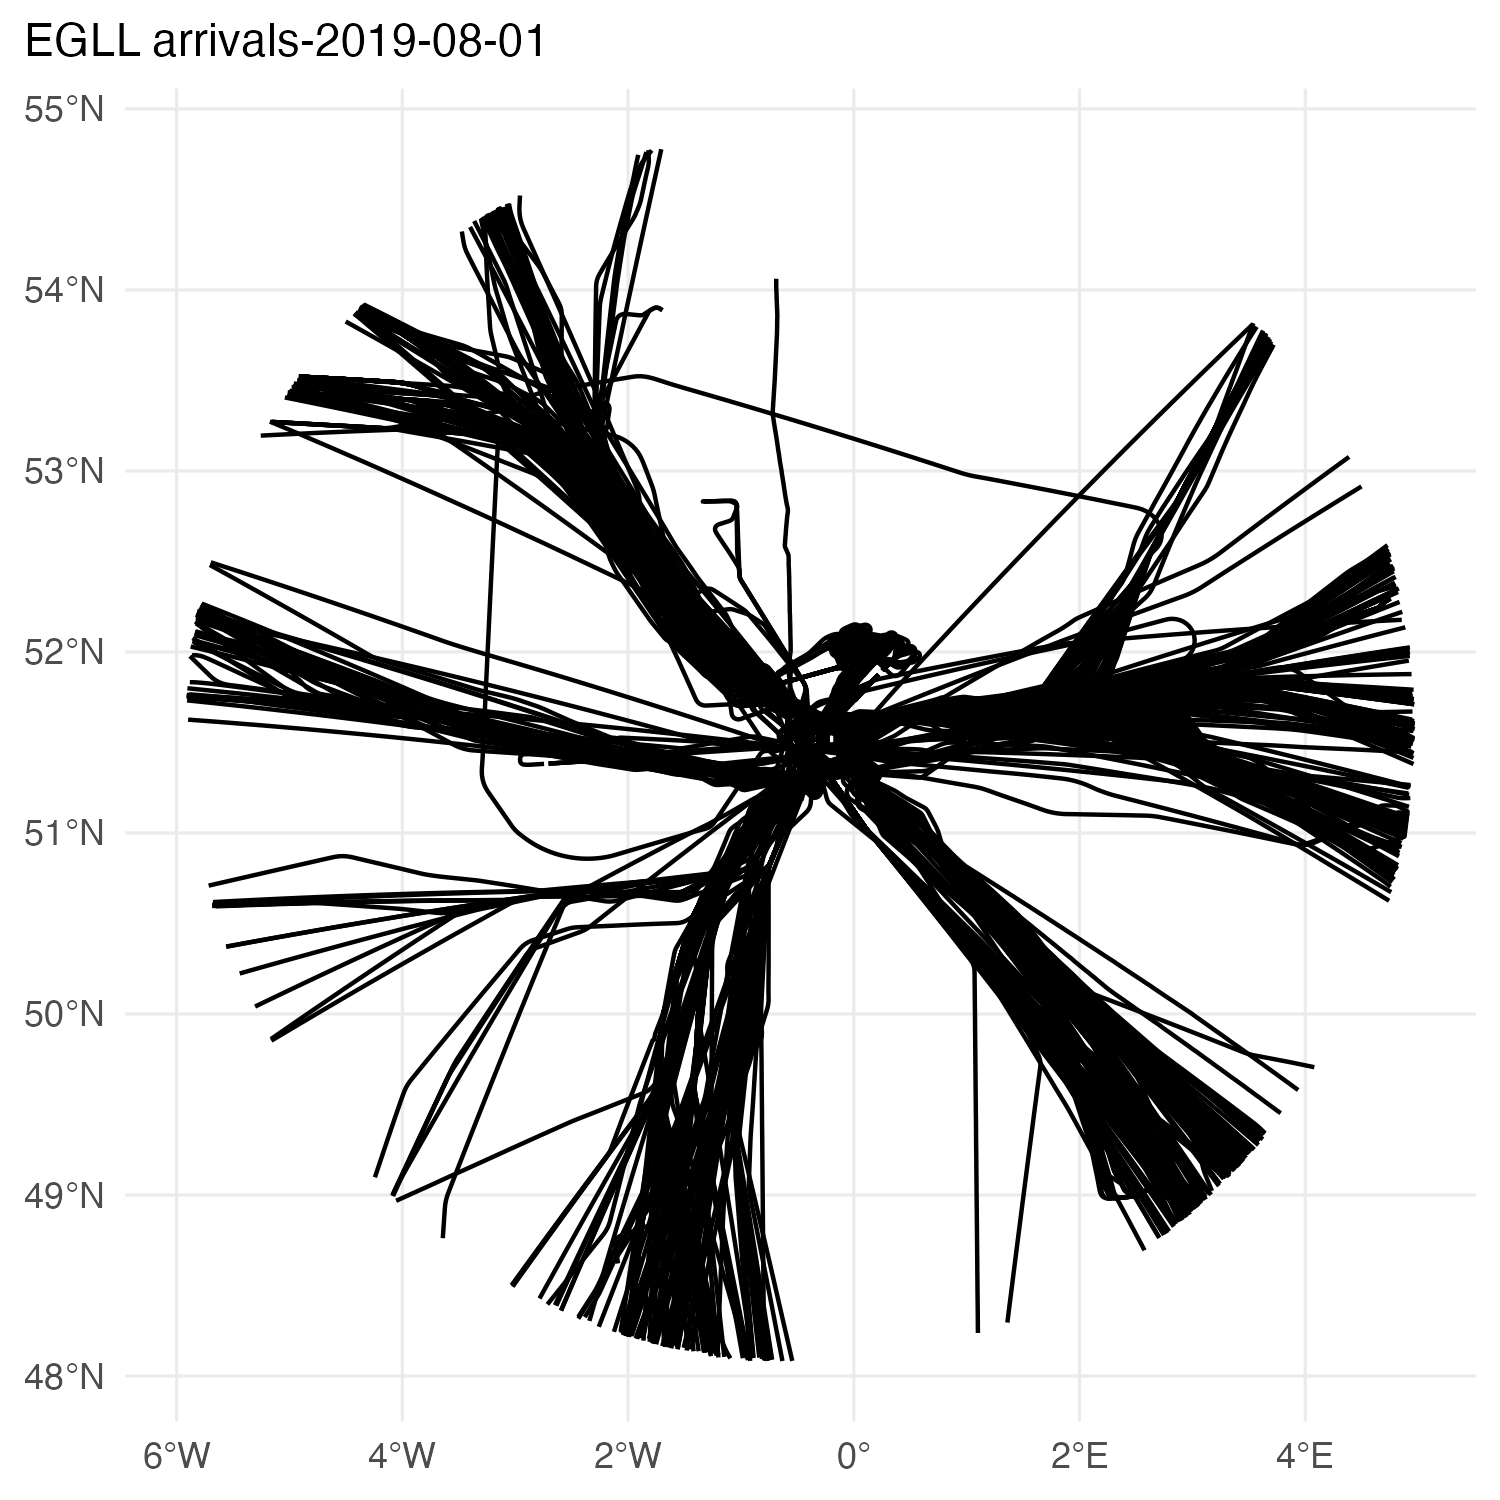
\includegraphics[width=0.45\textwidth,height=\textheight]{./figures/EGLL-arrivals-single-day.png}

}

\caption{\label{fig-EGLL-arrivals}Arrivals at London Heathrow (EGLL) on
sample day}

\end{figure}

\hypertarget{landing-runway-identification}{%
\subsubsection{Landing Runway
Identification}\label{landing-runway-identification}}

The identification of the landing direction is based on a simple
geospatial heuristic. Conceptually, aircraft are aligned with the runway
(centerline) before landing. An aircraft is assigned to a landing runway
based on the closeness of its pre-landing positions to the extended
runway centerline.

\begin{figure}

{\centering 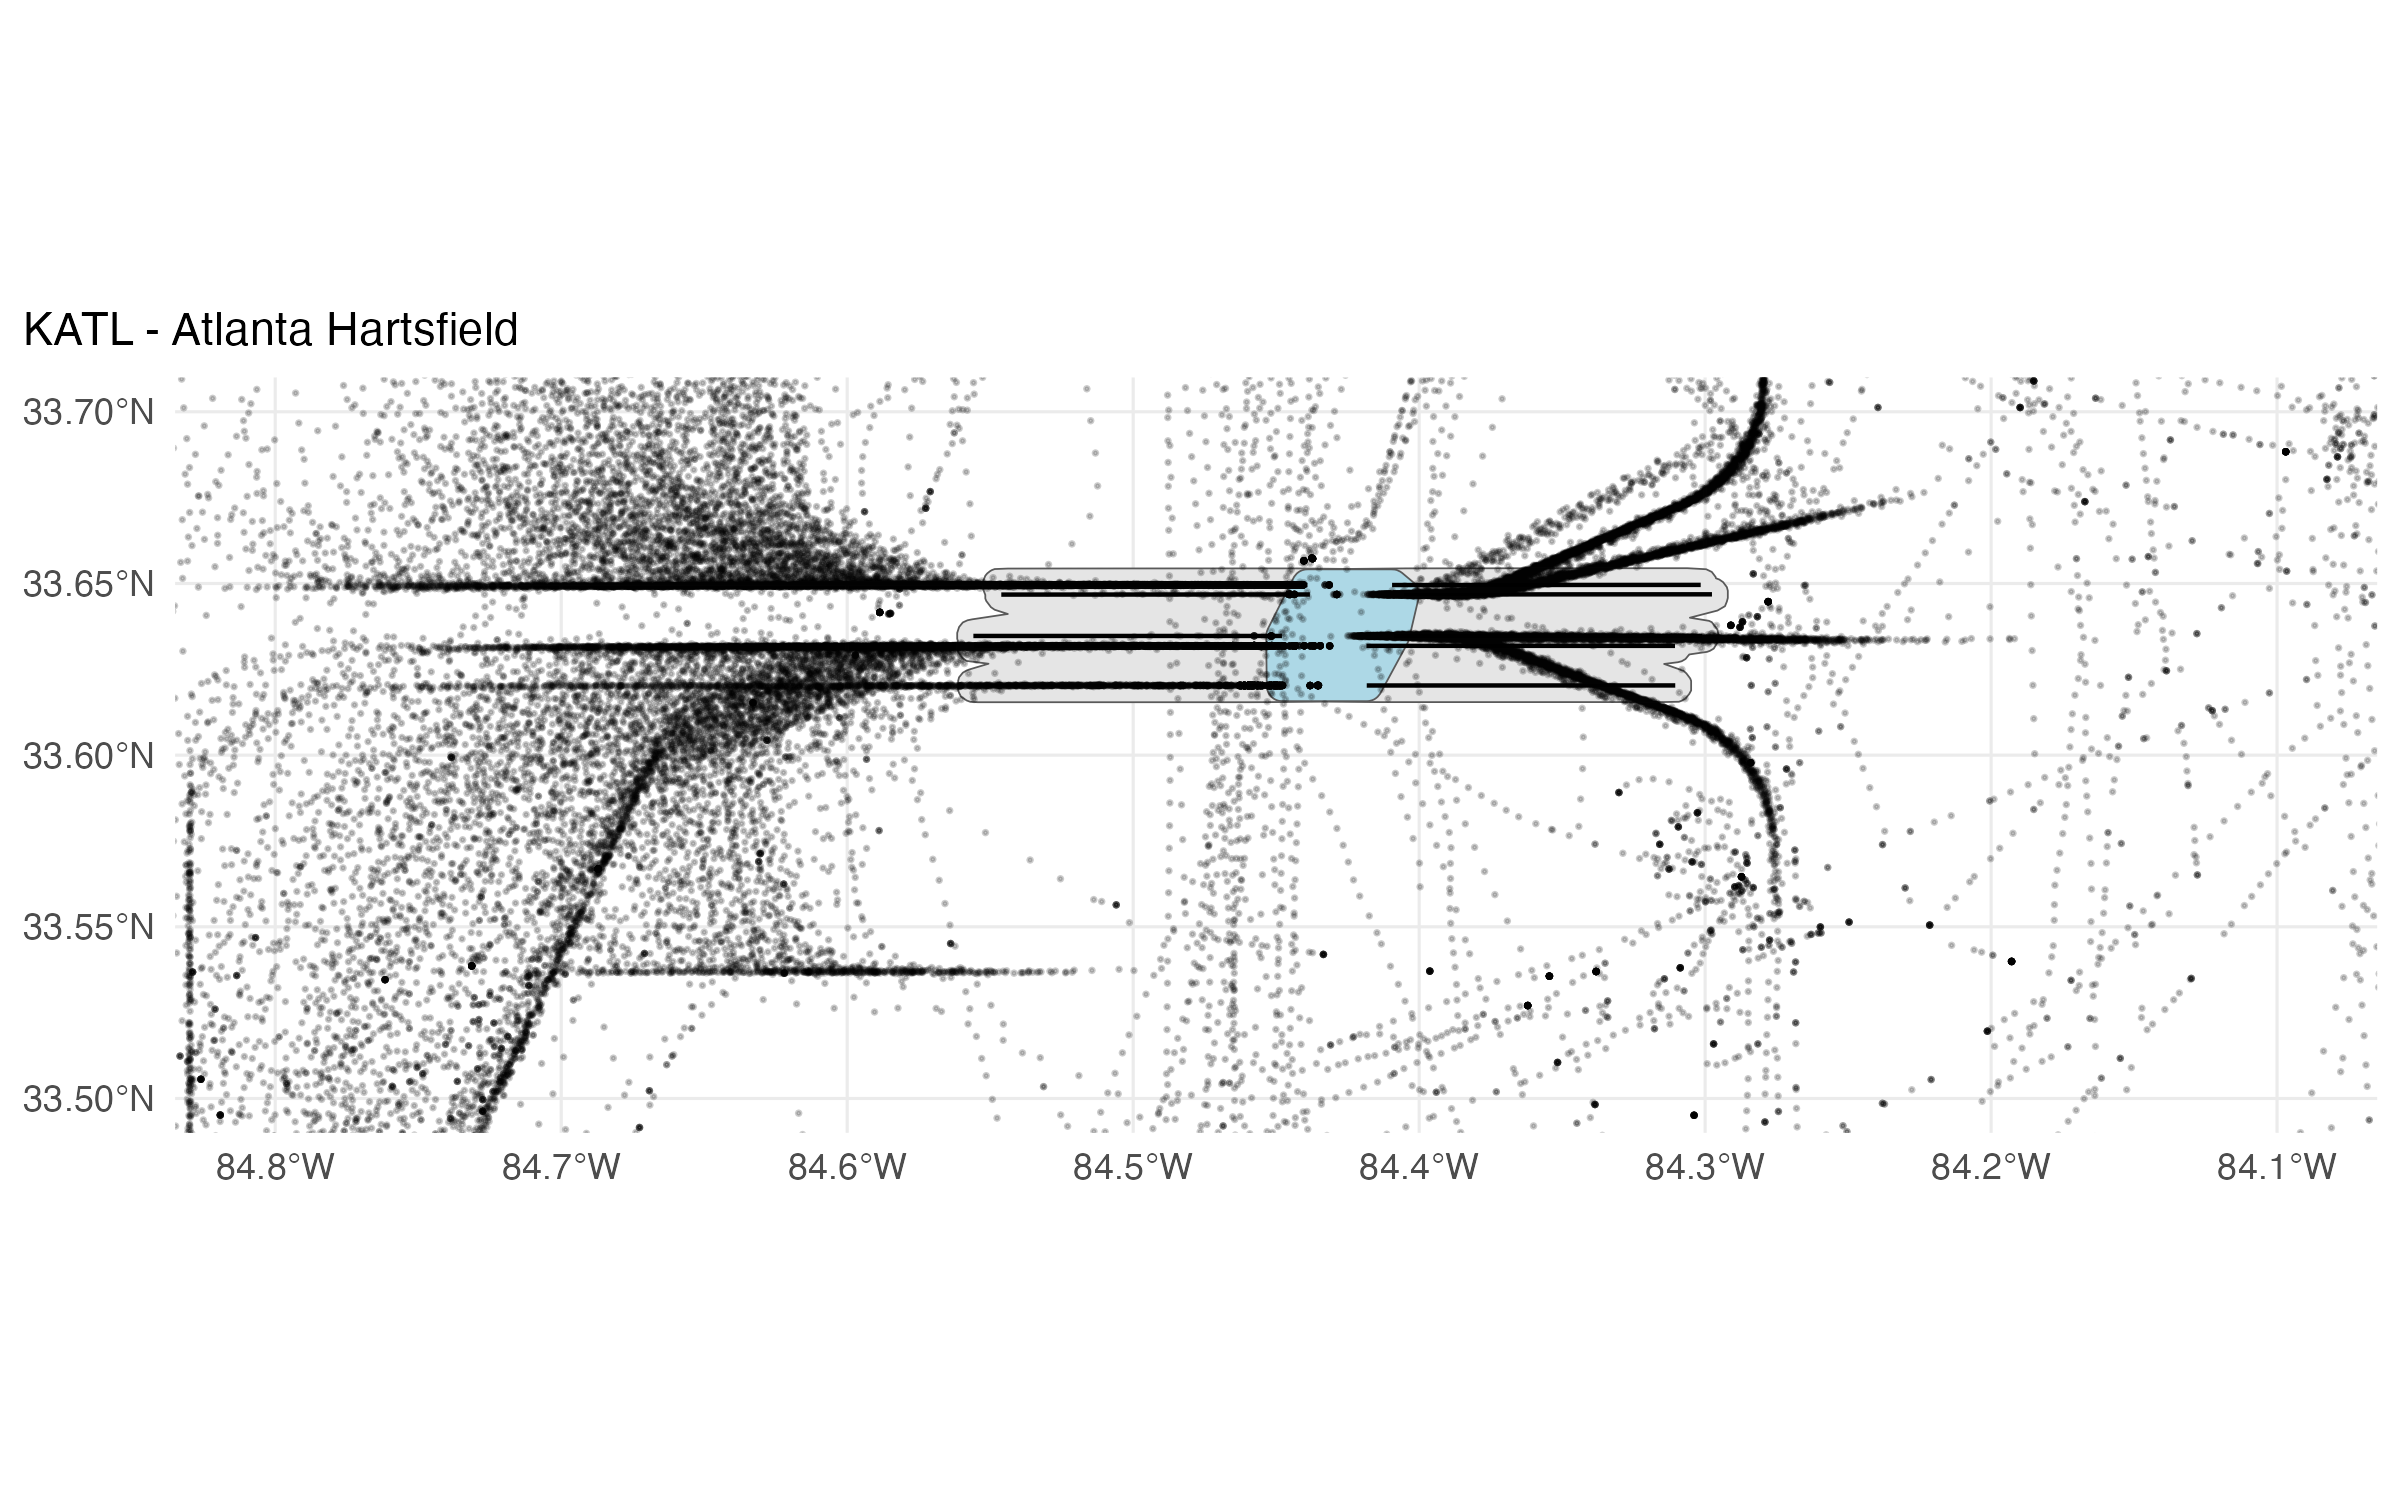
\includegraphics[width=0.45\textwidth,height=\textheight]{./figures/KATL-traffic-single-day.png}

}

\caption{\label{fig-KATL-arrivals}Arrivals at Atlanta Hartsfiled (KATL)
on sample day}

\end{figure}

\hypertarget{generalisation-of-additional-time-in-terminal-airspace}{%
\subsection{Generalisation of additional time in terminal
airspace}\label{generalisation-of-additional-time-in-terminal-airspace}}

The additional time in terminal airspace (c.f. ICAO KPI08, EUROCONTROL
Performance Review System \& European Single European Sky Performance
Scheme) is typically expressed as the difference between the observed
travel time of a flight entering the terminal area (e.g.~40NM or 100NM
from the aerodrome reference point) and a respective reference time. The
latter is defined as the travel time in non-congested situations. For
practical reasons, the reference (or uncongested) travel times are
determined based on a historical data analysis and sub-sampling the
population of arrival flights per entry sector/fix, aircraft wake
turbulence category and propulsion type (as a proxy of approach speed),
and landing runway.

This notion of additional time can be generalised for every subset of
points within the arrival airspace. On the basis of historic data, the
travel time between such a set of points can be determined and compared
to the flight time of an uncongested trajectory.

\begin{figure}

{\centering 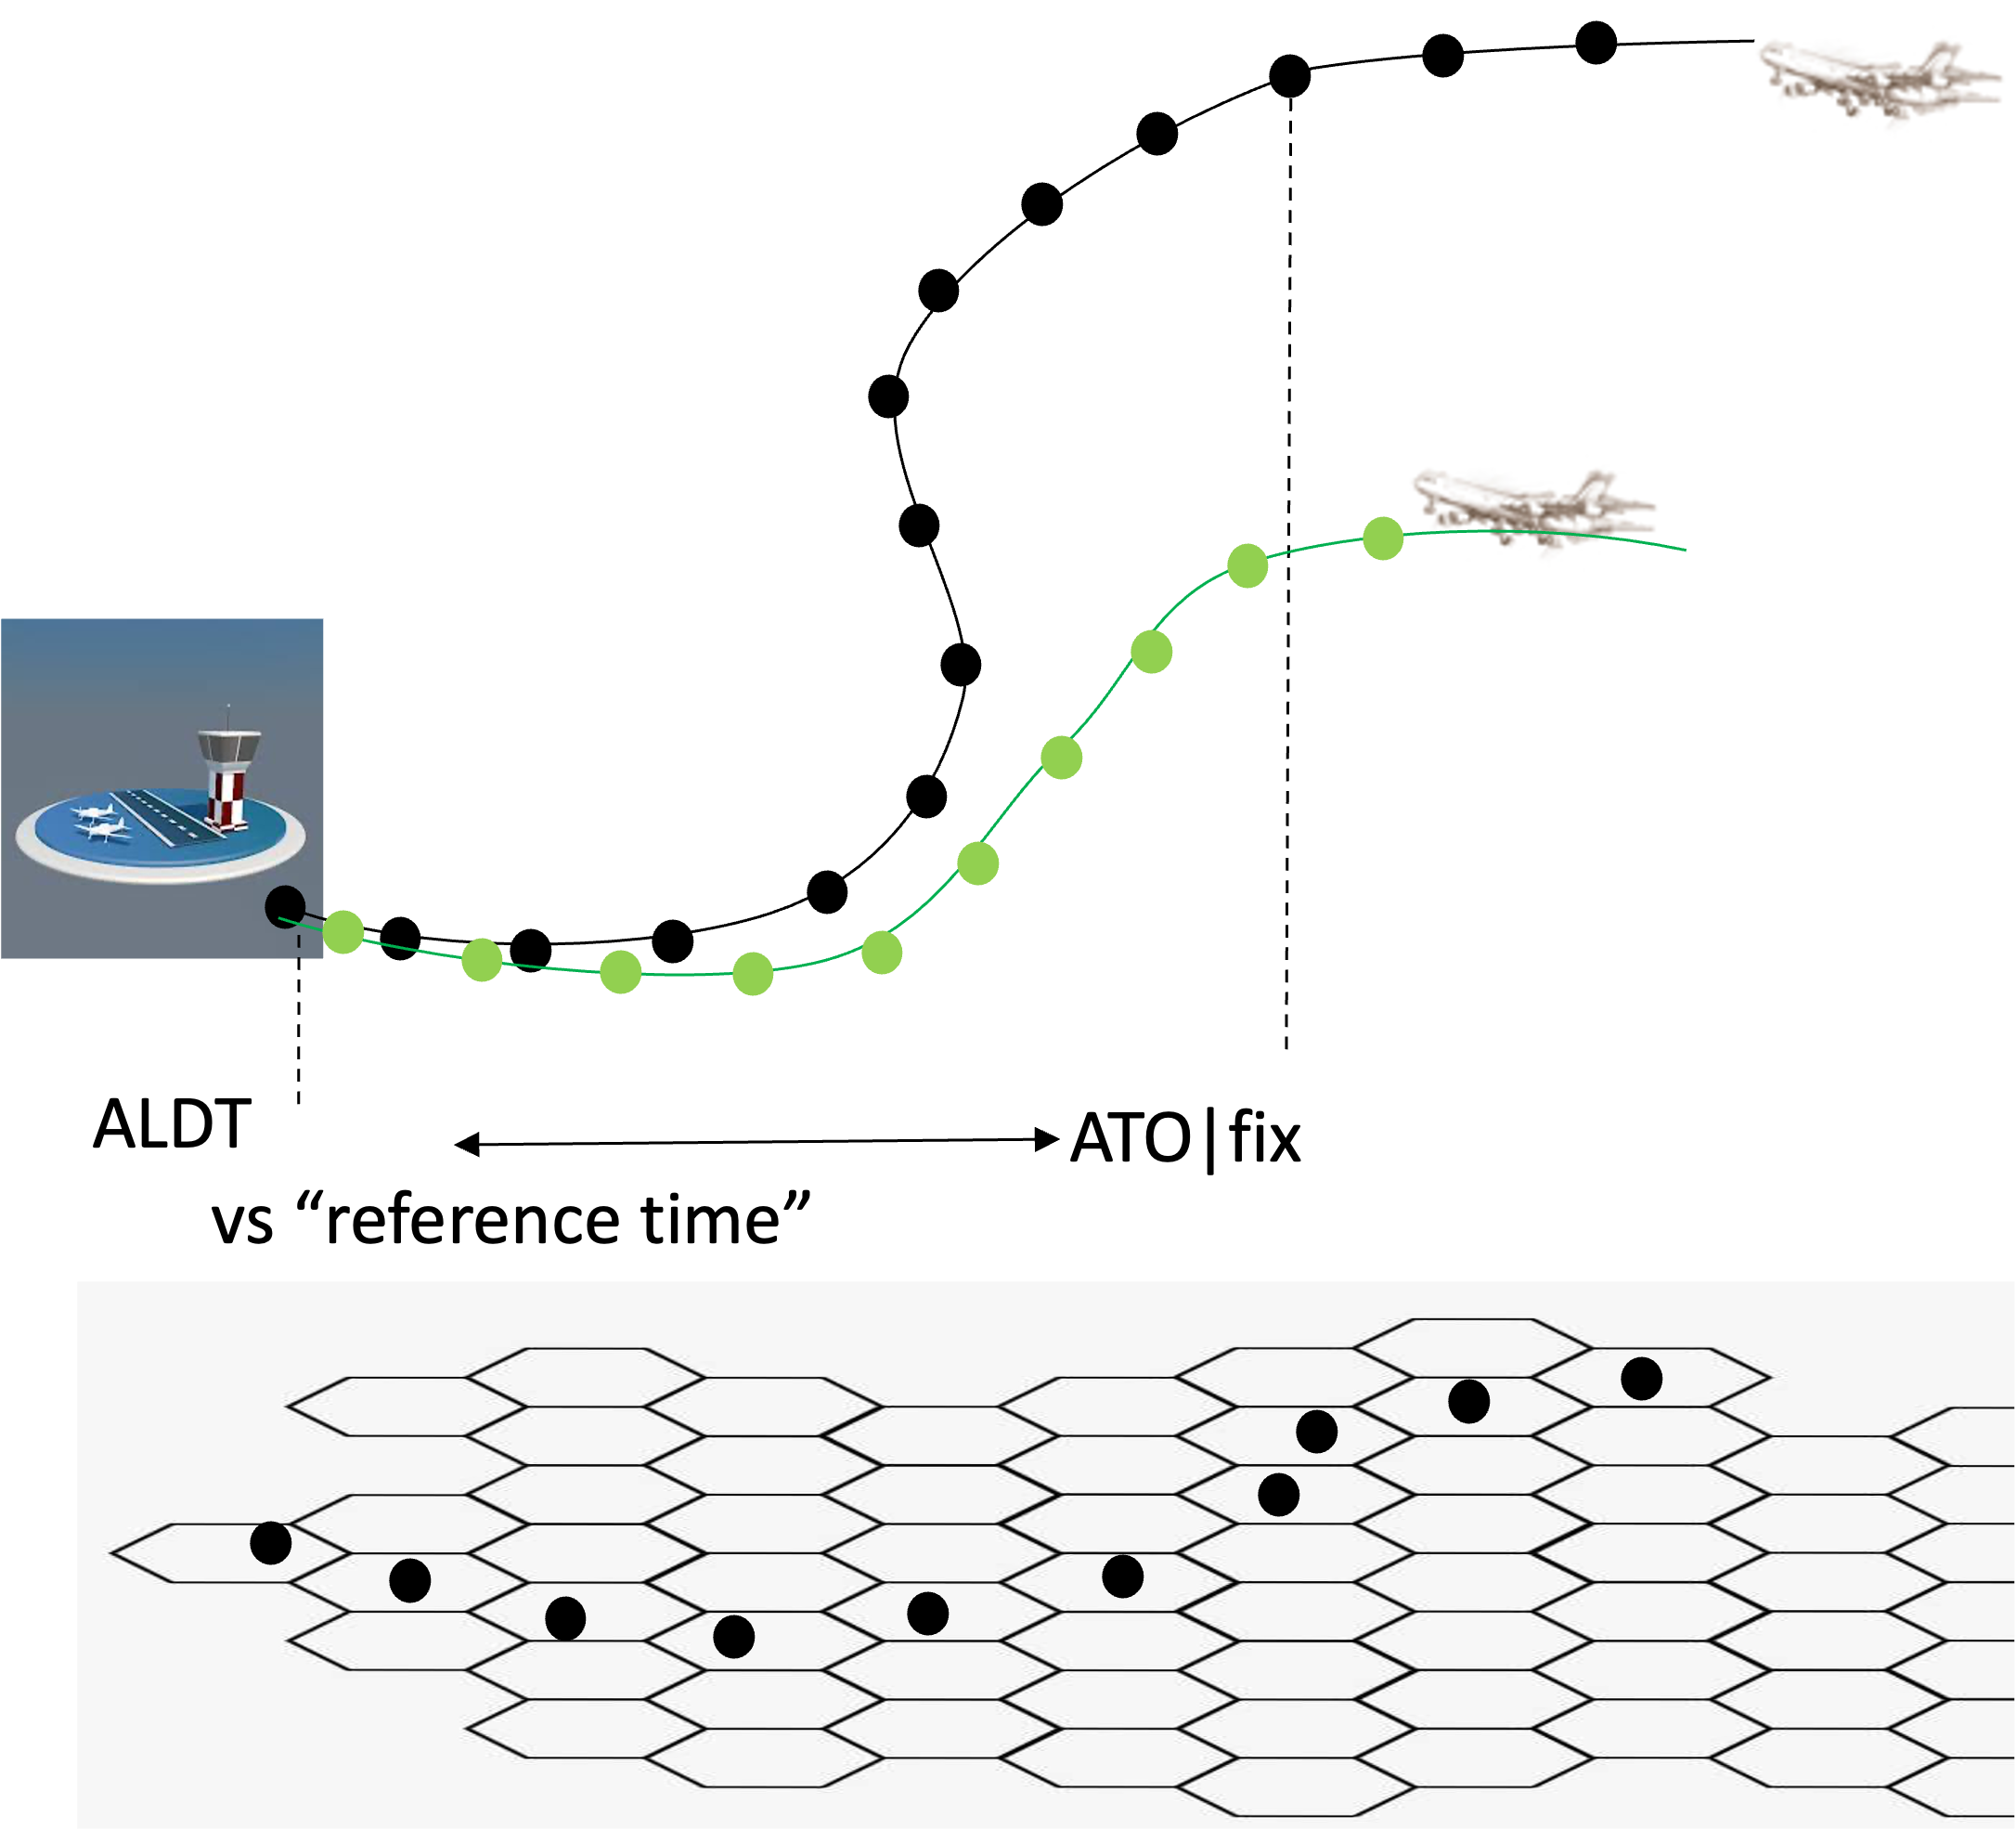
\includegraphics[width=0.45\textwidth,height=\textheight]{./figures/concept.png}

}

\caption{\label{fig-spacing-deviation-concept}Spacing deviation concept}

\end{figure}

For practical reasons, this paper discretises the arrival airspace into
cells. In particular, we are using hexogonal cells and the H3-indexing
system \protect\hyperlink{ref-ubertechnologiesinc2018}{{[}2{]}}. Uber
originally developed the Hexagonal Hierarchical Geospatial Indexing
System (H3) as a grid system for supporting the optimisation of ride
planning (and associated pricing and dispatch) and for visualisation
purposes. H3 is available as an open-source library written in C and
with bindings in several languages. We use hexagon-cells of resolution 8
with an average edge length of 0.5314 km.

\hypertarget{arrival-sequencing---spacing-deviation}{%
\subsection{Arrival Sequencing - Spacing
Deviation}\label{arrival-sequencing---spacing-deviation}}

Let us consider a pair of consecutive landing aircraft denoted leader
and trailer, with \(s\) being their temporal spacing (inter-arrival
time). From an operational perspective, highly efficient operations will
maximise the utilisation of the available runway (system) capacity.
Accordingly, we can assume that during peak times the temporal spacing
at landing \(s\) accounts for the operational concept applied at the
airport, and only comprises a minimal spacing error. Potential error
sources include additional safety margins applied by the air traffic
controller (or aircrew when landing under visual flight rules),
variations of the arrival spacing due to reduction of airspeed during
the flare. We consider the observed temporal spacing \(s_{ij}\) as a
lower bound for safe operations.

Using the constant time delay principle, the spacing deviation (or
spacing error) at time t considers the current position of trailer at
time \(t\), and the past position of leader at time \(t-s\). Based on
our approach, the spacing deviation is defined as the temporal
difference between the respective reference times for the position of
the leader and trailer:

\begin{equation}\protect\hypertarget{eq-spacing-deviation}{}{\begin{aligned}
spacing \text{ } deviation (t) =  ref{\_}time(trailer_{(t)}) - \\ref{\_}time(leader_{(t - s)})
\end{aligned}}\label{eq-spacing-deviation}\end{equation}

\begin{figure}

{\centering 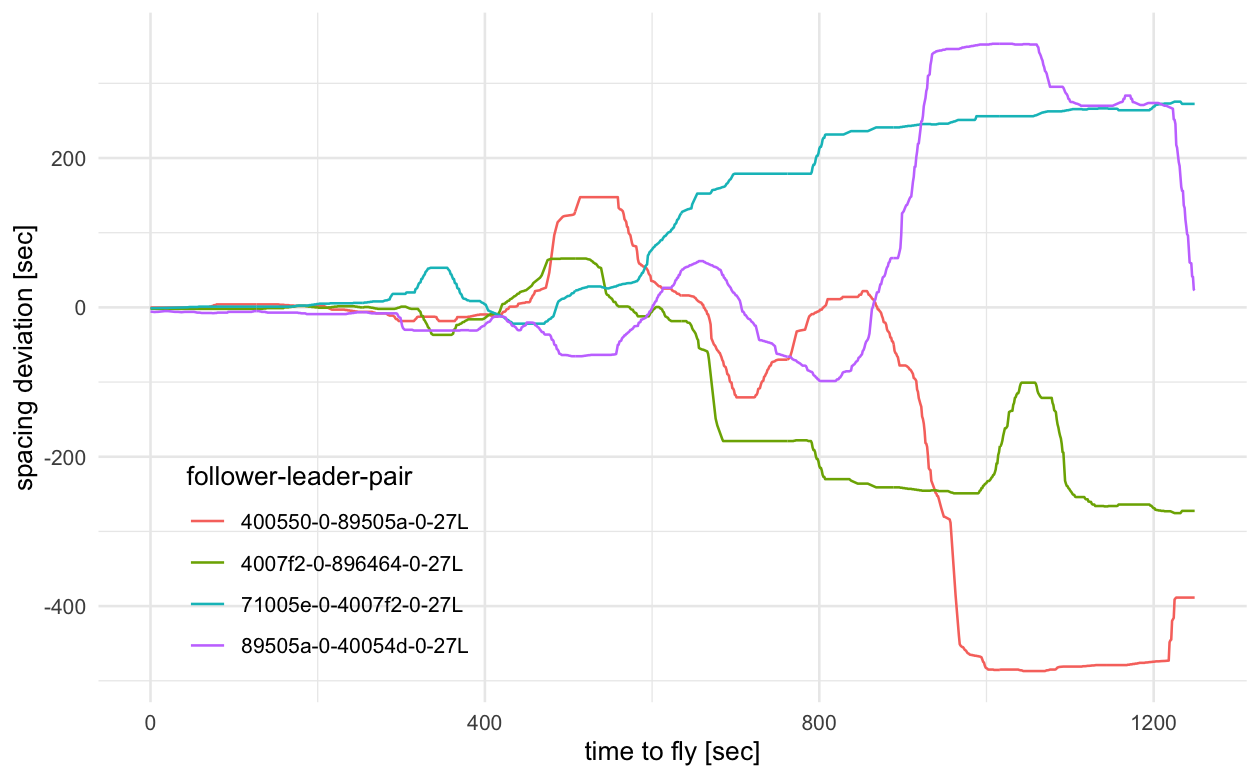
\includegraphics[width=0.45\textwidth,height=\textheight]{./figures/example-follower-leader-pairs.png}

}

\caption{\label{fig-follower-leader-example}Example timeline of spacing
deviations between interacting arrivals}

\end{figure}

Equation~\ref{eq-spacing-deviation} does something.

\hypertarget{case-study---results}{%
\section{Case Study - Results}\label{case-study---results}}

\hypertarget{data-sampling}{%
\subsection{Data Sampling}\label{data-sampling}}

At the time of writing no global open flight table exists. For this
study, we validated the sample with reference data available to the
Performance Review Unit. Under the EUROCONTROL Performance Review
System, airport operators report movement data on a monthly basis
\protect\hyperlink{ref-apdf_v1_2019}{{[}3{]}}.

\hypertarget{conclusions}{%
\section{Conclusions}\label{conclusions}}

Ambitious political targets for 2050 have been formulated to curb the
contribution of air transportation to climate change and work towards
climate neutrality. Policy and industry action revolve around a variety
of measures. Within this context - and in light of the required lead
time for a global pickup on sustainable aviation fuels, the introduction
of novel airframe designs, or propulsion technology - increasing the
operational efficiency is a declared now-term measure. There is a
substantial benefit pool for the wider arrival phase covering the
airspace within 200NM of the destination airport. Trajectory-based
operations promise higher levels of predictability and reduced
inefficiencies. The benefits of reducing spacing and flow
synchronisation measures in the terminal airspace are therefore
dependent on the capability of balancing out operational variations from
delivery of the aircraft to the wider arrival airspace.

This proof-of-concept paper aims at operationalising a performance
measure to characterise arrival management techniques, but also provide
a basis to discuss the handover from the enroute phase to the wider
arrival airspace.

This paper aimed at exploring a data-driven approach to measuring
operational efficiency during the arrival phase. In light of the ongoing
discussions about the climate impact of air transportation and the contr
Arrival management based on open data.

The proposed approach builds on the generalisation of a well-understood
key performance metric for the wider arrival airspace. It follows a
data-driven approach that is independent of detailed local context
modelling. For example, local airspace restrictions or procedures are
embedded in the temporal-spatial framework. Measuring the spacing
deviation between interacting arrival flights provides a basis for the
analysis of approach concepts that can help to streamline the arrival
sequencing and contribute to the further reduction of unnecessary fuel
burn and emissions.

This proof-of-concept addresses the aspect of transparency by making use
of openly available air transport trajectory data and open (analytical)
software. The approach is readily transferrable to other regions.

The goal of this work was the initial development of an operational
performance measure. Further validation is required at a larger set of
European (and global airports). This will allow for the refinement of
the parameterization of the approach. It is planned to roll-out the
approach under the umbrella of the EUROCONTROL Performance Review
System. This will provide European stakeholders with a means to address
enhancement of arrival operations, and may help to build a catalogue of
arrival management techniques that support higher levels of efficiency.

This paper demonstrated feasibility of the approach. While the proposed
performance monitoring of the spacing deviation envelope provides a
basis for identifying inefficiencies during the arrival flow, there is a
need to account also for factors driving and impacting the observed
performance. The temporal assessment of spacing deviation

\begin{itemize}
\tightlist
\item
  weather, wind
\item
  runway system configuration, adjacent aerodromes/level capping
\end{itemize}

On the algorithmic level, future work should address the impact of the
geospatial dimensions of cells and the method of their definition.

This paper applied a observational approach to determining the reference
times per cell. This will pose challenges for longer time horizons as
the continual update and processing of arrival trajectories would
require substantial resources. A possibility is the use of data
structures to support the continual online accumulation of statistics
without the need to store the complete historic dataset or processed
artefacts.

The results demonstrate the general feasibility of the approach. The
proposed approach offers a measure to start the dialogue between
operational planners and stakeholders to identify benefit pools during
the arrival phase.

\hypertarget{reproducibility}{%
\section*{Reproducibility}\label{reproducibility}}
\addcontentsline{toc}{section}{Reproducibility}

This paper has been built with the R/RStudio ecosystem. The draft
manuscript and its supporting data preparatory steps are archived at
https://github.com/rainer-rq-koelle/paper-2023-ICNS.

\hypertarget{acknowledgment-and-disclaimer}{%
\section*{Acknowledgment and
Disclaimer}\label{acknowledgment-and-disclaimer}}
\addcontentsline{toc}{section}{Acknowledgment and Disclaimer}

The authors thank the comments by colleagues from the Performance
Section of the Department of Airspace Control (DECEA) Brazil and the
Performance Review Unit of EUROCONTROL. This study would have not been
feasible without the generous support of Opensky Network and the many
community members collecting and feeding open ADSB data.

The views expressed are the authors' own and do not represent a policy
or position of DECEA or EUROCONTROL .

\hypertarget{bibliography}{%
\section*{References}\label{bibliography}}
\addcontentsline{toc}{section}{References}

\hypertarget{refs}{}
\begin{CSLReferences}{0}{0}
\leavevmode\vadjust pre{\hypertarget{ref-sun2017flightphase}{}}%
\CSLLeftMargin{{[}1{]} }%
\CSLRightInline{J. Sun, J. Ellerbroek, and J. Hoekstra, {``Flight
extraction and phase identification for large automatic dependent
surveillance\textendash broadcast datasets,''} \emph{Journal of
Aerospace Information Systems}, vol. 14, no. 10, pp. 566--572, 2017. }

\leavevmode\vadjust pre{\hypertarget{ref-ubertechnologiesinc2018}{}}%
\CSLLeftMargin{{[}2{]} }%
\CSLRightInline{Uber Technologies Inc, {``H3: Hexagonal hierarchical
geospatial indexing system.''} 2018 {[}Online{]}. Available:
\url{https://h3geo.org/}}

\leavevmode\vadjust pre{\hypertarget{ref-apdf_v1_2019}{}}%
\CSLLeftMargin{{[}3{]} }%
\CSLRightInline{EUROCONTROL, {``Eurocontrol {Specification} for
{Operational ANS Performance Monitoring} - {Airport Operator Data
Flow}.''} 2019 {[}Online{]}. Available:
\url{https://www.eurocontrol.int/publication/eurocontrol-specification-operational-ans-performance-monitoring}}

\end{CSLReferences}

% done
\end{document}
